%----------------------------------------------------------------------------------------
%    PACKAGES AND THEMES
%----------------------------------------------------------------------------------------

\documentclass[aspectratio=169,xcolor=dvipsnames]{beamer}
\usetheme{SimplePlus}

\usepackage{tikz}
\usepackage{hyperref}
\usepackage{graphicx} % Allows including images
\usepackage{booktabs} % Allows the use of \toprule, \midrule and \bottomrule in tables
\usepackage{wrapfig}
\usepackage{listings}
\usepackage[font=small,labelfont=bf]{caption}

%----------------------------------------------------------------------------------------
%    TITLE PAGE
%----------------------------------------------------------------------------------------

\title{Classification 2}
\subtitle{HI 743}

\author{Ryan Gallagher}

\institute
{
    Department of Health Informatics and Administration \\
    Zilber College of Public Health \\
    University of Wisconsin - Milwaukee% Your institution for the title page
}
\date{Match 6th, 2025} % Date, can be changed to a custom date


%----------------------------------------------------------------------------------------
%    PRESENTATION SLIDES
%----------------------------------------------------------------------------------------

\begin{document}
\begin{frame}
    % Print the title page as the first slide
    \titlepage
\end{frame}

%----------------------------------------------------------------------------------------
%    Outline
%----------------------------------------------------------------------------------------

\begin{frame}{Overview}
    % Throughout your presentation, if you choose to use \section{} and \subsection{} commands, these will automatically be printed on this slide as an overview of your presentation
    \tableofcontents
\end{frame}

%----------------------------------------------------------------------------------------
%    Slides
%----------------------------------------------------------------------------------------
\section{K-Nearest Neighbors}
% Slide 27: Introduction to K-Nearest Neighbors
\begin{frame}{K-Nearest Neighbors (KNN)}
    \textbf{A Non-Parametric Classification (Linear) Method}
    \begin{itemize}
    \setlength\itemsep{0.5cm}
        \item KNN classifies a test observation based on the majority class among its \( K \) closest neighbors.
        \item No explicit parametric assumptions about the data. Data does not have to be linearly related.
        \item Can be used for both classification and regression tasks. Both continuous (numeric) or categorical outcomes are permitted. We will focus on classification.
    \end{itemize}
\end{frame}

% Slide 28: KNN Algorithm
\subsection{Algorithm}
\begin{frame}{KNN Algorithm}
    \textbf{Steps in KNN:}
    \begin{enumerate}
        \setlength\itemsep{0.33cm}
        \item Choose the number of neighbors \( K \).
        \item Compute the distance between the test observation and all training observations.
        \item Identify the \( K \) nearest neighbors.
        \item Assign the most common class label among the neighbors (majority vote).
    \end{enumerate}
    \begin{figure}
        \centering
        %\includegraphics[width=0.6\linewidth]{knn_diagram.png}
        %\caption{Illustration of KNN with different values of \( K \).}
    \end{figure}
\end{frame}
\subsection{KNN Example}
% Slide 28.5: KNN Example from ISL
\begin{frame}{Example: KNN Classification}
    \textbf{Illustrative Example from ISL}
    \begin{itemize}
        \item Consider a dataset with two classes: blue and orange.
        \item A new test observation (black cross) is classified using KNN with \( K = 3 \).
        \item The three closest points (circled) are identified.
        \item Since two out of three neighbors are blue, the test observation is classified as blue.
    \end{itemize}
    \begin{figure}
        \centering
        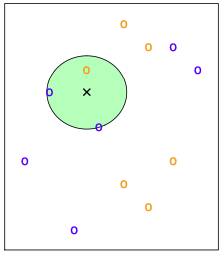
\includegraphics[width=0.25\linewidth]{images/circle.png}
        \caption{KNN classification example from ISL.}
    \end{figure}
\end{frame}

% Slide 28.6: KNN Decision Boundary Example
\begin{frame}{KNN Decision Boundary}
    \begin{itemize}
        \item The decision boundary separates the feature space into regions assigned to each class.
        \item When \( K \) is small, the boundary is highly flexible and follows training data closely.
        \item When \( K \) is large, the boundary becomes smoother and generalizes better.
    \end{itemize}
    \begin{figure}
        \centering
       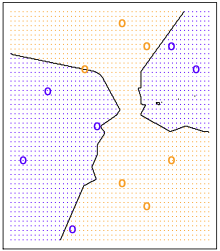
\includegraphics[width=0.3\linewidth]{images/classifier.png}
        \caption{KNN decision boundary for \( K = 3 \).}
    \end{figure}
\end{frame}

% Slide 29: Effect of K on KNN
\subsection{Choosing K}
\begin{frame}{Choosing K in KNN}
    \begin{itemize}
        \item \textbf{Small K:} High variance, low bias (overfits to noise in the data).
        \item \textbf{Large K:} Low variance, high bias (oversmooths the decision boundary).
        \item The optimal \( K \) is typically chosen using cross-validation.
    \end{itemize}
    \begin{figure}
        \centering
        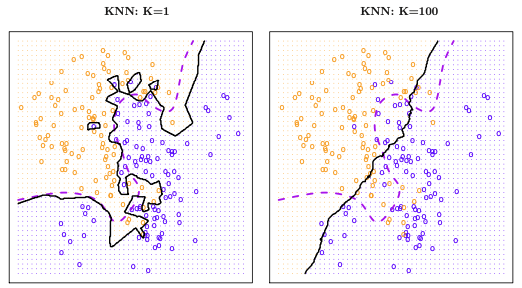
\includegraphics[width=0.6\linewidth]{images/boundary.png}
        \caption{Effect of different values of \( K \) on decision boundary.}
    \end{figure}
\end{frame}

% Slide 28.7: KNN Error Rate
\begin{frame}{KNN Error Rate Analysis}
    \textbf{Understanding the Impact of K on Error Rate}
    \begin{itemize}
        \item The classification error rate measures how often KNN misclassifies observations.
        \item Error rate varies with K:
        \begin{itemize}
            \item Small K: High variance, low bias, more sensitive to noise.
            \item Large K: Low variance, high bias, smoother boundaries.
        \end{itemize}
        \item The optimal K minimizes the test error rate.
    \end{itemize}
    \begin{figure}
        \centering
        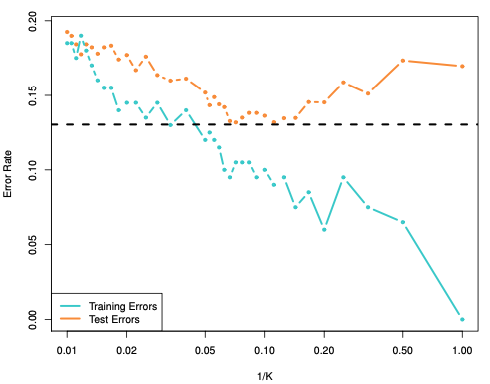
\includegraphics[width=0.3\linewidth]{images/knn_error_rate.png}
        \caption{KNN error rate for different values of K.}
    \end{figure}
\end{frame}

% Slide 30: Strengths and Weaknesses of KNN
\begin{frame}{Strengths and Weaknesses of KNN}
    \textbf{Strengths:}
    \begin{itemize}
        \item Simple and intuitive.
        \item Works well with small datasets.
    \end{itemize}
    \textbf{Weaknesses:}
    \begin{itemize}
        \item Computationally expensive for large datasets.
        \item Performance depends on the choice of distance metric.
        \item Sensitive to irrelevant or redundant features.
    \end{itemize}
\end{frame}

\section{K-Means Clustering}
\subsection{Algorithm}
% Slide 31: Introduction to K-Means Clustering
\begin{frame}{K-Means Clustering}
    \textbf{A Partitioning Clustering Method}
    \begin{itemize}
    	\setlength\itemsep{0.33cm}
	\item An unsupervised machine learning method.
        \item K-means clustering partitions observations into \( K \) distinct clusters.
        \item Each cluster is defined by its \textbf{centroid} (mean of points in that cluster).
        \item The goal is to minimize within-cluster variation - i.e. to make the observations within each cluster be as similar as possible.
    \end{itemize}
\end{frame}

% Slide 32: K-Means Algorithm
\begin{frame}{K-Means Algorithm}
    \textbf{Steps in K-Means Clustering:}
    \begin{enumerate}
        \item Choose the number of clusters \( K \).
        \item Randomly assign each observation to one of the \( K \) clusters.
        \item Iterate until convergence:
        \begin{itemize}
            \item Compute the centroid of each cluster.
            \item Assign each observation to the nearest centroid.
        \end{itemize}
    \end{enumerate}
    \begin{figure}
        \centering
        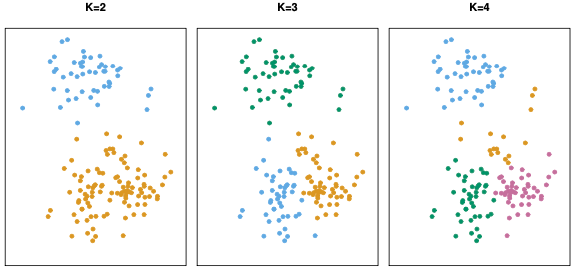
\includegraphics[width=0.55\linewidth]{images/kmeans_algorithm.png}
        \caption{Illustration of K-Means clustering process.}
    \end{figure}
\end{frame}

% Slide 32.5: Graphics
\begin{frame}{K-Means Algorithm}
\begin{figure}
\centering
\includegraphics[width=0.48\linewidth]{images/kmeans_graphic.png}
\end{figure}
\end{frame}

\subsection{Evaluation}
% Slide 34: Evaluating K-Means Clustering
\begin{frame}{Evaluating K-Means Clustering}
    \textbf{Metrics for Clustering Performance:}
    \begin{itemize}
        \item Within-cluster variation: Measures how tight clusters are.
        \item Total within-cluster sum of squares (WCSS): Sum of squared distances from each point to its cluster centroid.
        \item Between-cluster variation: Measures how well-separated clusters are.
        \item Elbow Method: A common technique to select the optimal \( K \).
    \end{itemize}
    \begin{figure}
        \centering
        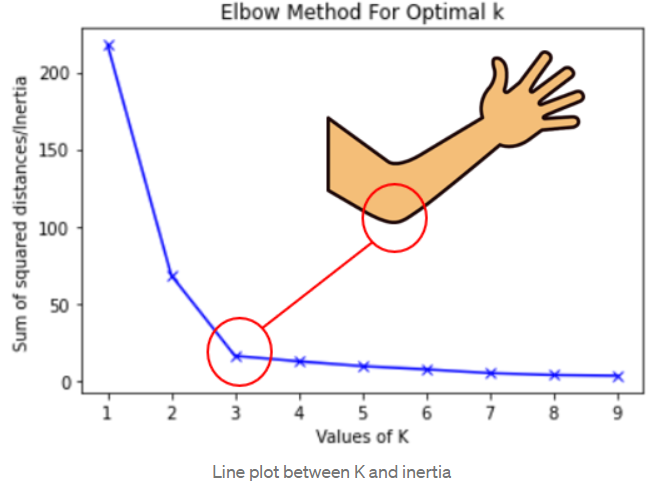
\includegraphics[width=0.4\linewidth]{images/elbow.png}
        \caption{Elbow Method for selecting optimal \( K \).}
    \end{figure}
\end{frame}

% Slide 35: Applications of K-Means Clustering
\begin{frame}{Applications of K-Means Clustering}
    \textbf{Real-World Uses of K-Means Clustering:}
    \begin{itemize}
    \setlength\itemsep{0.33cm}
        \item Healthcare:
        \begin{itemize}
            \item Patient segmentation for personalized treatments.
            \item Disease subtype identification based on genetic markers.
        \end{itemize}
        \item Marketing \& Customer Segmentation:
        \begin{itemize}
            \item Identifying customer groups for targeted advertising.
            \item Analyzing purchasing behavior.
        \end{itemize}
        \item Social Network Analysis:
        \begin{itemize}
            \item Community detection in large networks.
            \item Recommender systems for user-group clustering.
        \end{itemize}
    \end{itemize}
\end{frame}


\end{document}